\begin{figure}[H]
    \centering
    % First plot
    \begin{minipage}{0.48\textwidth}
        \centering
        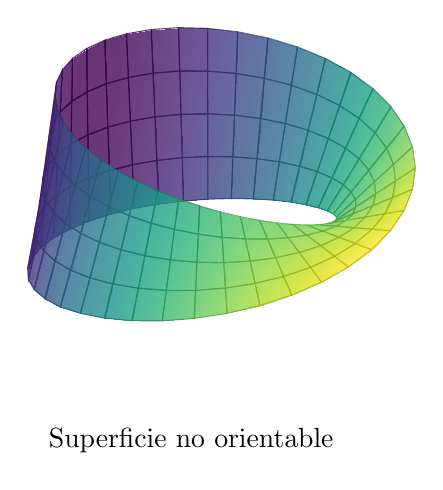
\begin{tikzpicture}
            \begin{axis}[
                hide axis,
                view = {40}{40},
                colormap/viridis,
            ]
                \addplot3 [
                    surf,
                    colormap/viridis,
                    shader     = faceted interp,
                    point meta = x,
                    samples    = 40,
                    samples y  = 5,
                    z buffer   = sort,
                    domain     = 0:360,
                    y domain   = -0.5:0.5,
                    opacity=0.8
                ] (
                    {(1+0.5*y*cos(x/2)))*cos(x)},
                    {(1+0.5*y*cos(x/2)))*sin(x)},
                    {0.5*y*sin(x/2)}
                );
            \end{axis}
            \node[below] at (3,0) {Superficie no orientable};
        \end{tikzpicture}
    \end{minipage}
    \hfill
    % Second plot
    \begin{minipage}{0.48\textwidth}
        \centering
        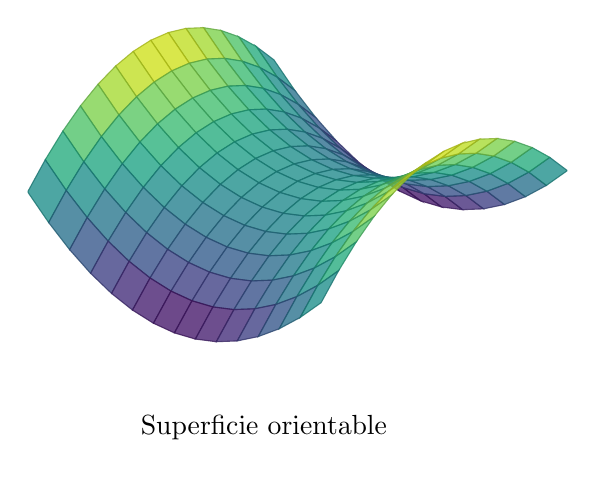
\begin{tikzpicture}
            \begin{axis}[
                hide axis,
                view={40}{40},
                colormap/viridis
            ]
                \addplot3[
                    surf,
                    opacity=0.8,
                    domain=-2:2,
                    samples=15
                ] {x^2 - y^2};
            \end{axis}
            \node[below] at (3,0) {Superficie orientable};
        \end{tikzpicture}
    \end{minipage}
\end{figure}

